% One week through the pipeline: nothing reaches a .bib without resolving.
% ---------------------------------------------------------------------------
% style.tex --- shared preamble for every figure in book/figures/tikz/
%
% One style for all figures: Latin Modern, thin black lines, a light grey
% fill, and one accent colour used only to mark what is untrusted or wrong.
% Build with scripts/build_figures.sh; see book/figures/README.md.
% ---------------------------------------------------------------------------
\documentclass[tikz,border=6pt]{standalone}
\usepackage[T1]{fontenc}
\usepackage{lmodern}
\usetikzlibrary{arrows.meta,positioning,shapes.geometric,calc,fit,backgrounds}

\hyphenpenalty=10000   % short lines in boxes: ragged, never hyphenated

\definecolor{lightgrey}{gray}{0.92}
\definecolor{accent}{HTML}{9B2D20}

\tikzset{
  every picture/.style={
    line width=0.6pt,
    font=\small,
    >={Stealth[length=5pt,width=4pt]},
    node distance=14pt and 24pt,
  },
  % shapes
  box/.style={draw, rectangle, inner xsep=8pt, inner ysep=5pt,
              minimum height=22pt, align=center},
  grey/.style={box, fill=lightgrey},
  rounded/.style={box, rounded corners=9pt},
  decision/.style={draw, diamond, aspect=2.4, inner sep=1.5pt, align=center},
  group/.style={draw, dashed, rounded corners=5pt, inner sep=7pt},
  % text
  tag/.style={font=\footnotesize, align=center, inner sep=2pt},
  note/.style={font=\footnotesize\itshape, align=center, inner sep=2pt},
  code/.style={font=\small\ttfamily},
  codetag/.style={font=\footnotesize\ttfamily, align=center, inner sep=2pt},
  title/.style={font=\small\scshape, align=center, inner sep=2pt},
  % lines
  arrow/.style={->},
  back/.style={->, dashed},
  thin/.style={line width=0.4pt, gray},
  % the one accent, for what is untrusted, wrong or missing
  bad/.style={accent},
  badbox/.style={box, draw=accent, text=accent},
}

\begin{document}
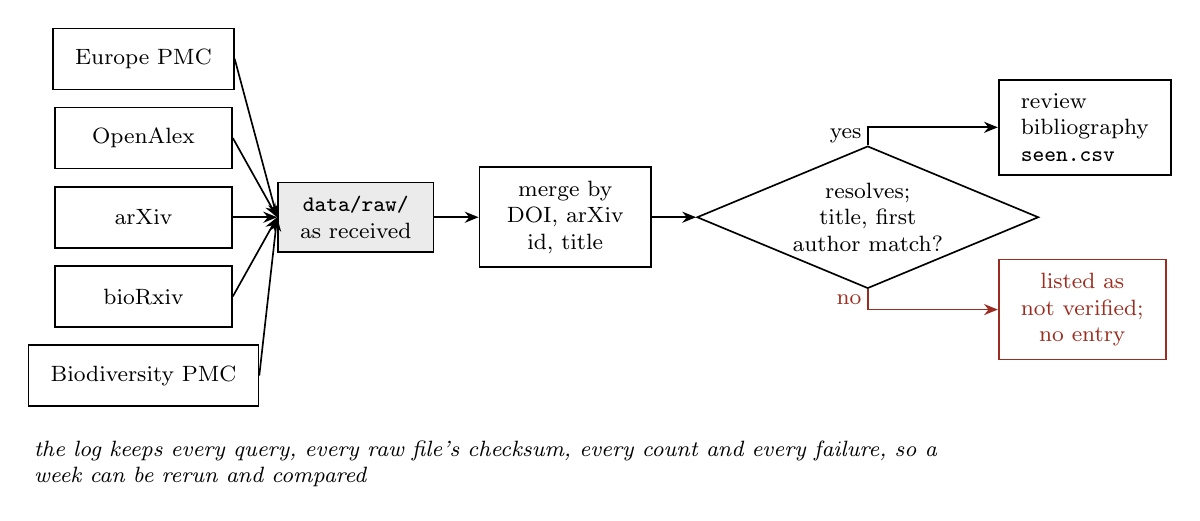
\begin{tikzpicture}[node distance=6pt and 16pt, src/.style={box, font=\footnotesize, minimum width=64pt, inner ysep=3pt}]
  \node[src] (s1) {Europe PMC};
  \node[src, below=of s1] (s2) {OpenAlex};
  \node[src, below=of s2] (s3) {arXiv};
  \node[src, below=of s3] (s4) {bioRxiv};
  \node[src, below=of s4] (s5) {Biodiversity PMC};
  \node[grey, right=of s3, font=\footnotesize, align=center] (raw) {\texttt{data/raw/}\\as received};
  \foreach \s in {s1,s2,s3,s4,s5} \draw[->] (\s.east) -- (raw.west);
  \node[box, right=of raw, text width=46pt, align=center, font=\footnotesize] (norm) {merge by DOI, arXiv id, title};
  \node[decision, right=of norm, font=\footnotesize] (q) {resolves;\\title, first\\author match?};
  \node[box, above right=2pt and 16pt of q, font=\footnotesize, align=left] (ok) {review\\bibliography\\\texttt{seen.csv}};
  \node[badbox, below right=2pt and 16pt of q, font=\footnotesize, align=center] (bad) {listed as\\not verified;\\no entry};
  \draw[->] (raw) -- (norm);
  \draw[->] (norm) -- (q);
  \draw[->] (q) |- node[tag, pos=0.25, left] {yes} (ok);
  \draw[->, bad] (q) |- node[tag, pos=0.25, left, text=accent] {no} (bad);
  \node[note, below=10pt of s5.south west, anchor=north west, text width=330pt, align=left]
    {the log keeps every query, every raw file's checksum, every count and every failure, so a week can be rerun and compared};
\end{tikzpicture}
\end{document}
